
%(BEGIN_QUESTION)
% Copyright 2012, Tony R. Kuphaldt, released under the Creative Commons Attribution License (v 1.0)
% This means you may do almost anything with this work of mine, so long as you give me proper credit

Suppose you were laying out the forms for a house foundation, and had to ensure the corners were ``square'' (exactly 90$^{o}$):

$$
\includegraphics[width=15.5cm]{i02678x01.eps}$$

How could you ensure this, using trigonometry?  How would you ensure this if you had no calculator with you to calculate trig functions, and no protractor or framing square with you to measure angles?  

\vskip 10pt

{\it Hint: remember that the lengths 3-4-5 happen to form a right triangle!}

\underbar{file i02678}
%(END_QUESTION)





%(BEGIN_ANSWER)

Using two adjacent sides of the foundation form, measure the diagonal and calculate whether its length is equal to the length of the hypotenuse for a right triangle.

\vskip 10pt

To do this with no calculator and with no angle-measuring tools, you could mark lengths along the two sides of the form equal to multiples of 3 and 4, then measure a diagonal length between those end points to see if it was equal to the same multiple of 5:

$$\includegraphics[width=15.5cm]{i02678x02.eps}$$

%(END_ANSWER)





%(BEGIN_NOTES)


%INDEX% Mathematics review: trigonometric calculations

%(END_NOTES)


